\part{Removendo o intermediário}
\label{ch:capitulo2}
\chapter*{Removendo o intermediário}

No capítulo anterior, comentamos que o Bitcoin fornece um sistema ponto a ponto para a transferência de valor. Antes de nos aprofundarmos em como isso funciona, vamos primeiro entender como um banco tradicional ou empresa de pagamento lida com o rastreamento da propriedade e das transferências de ativos.

\paragraph{Os bancos são apenas livros contábeis}
\paragraph{}

Como funciona um pagamento digital feito por seu banco, PayPal ou ApplePay? Muito simples, essas entidades intermediárias têm um livro-razão de contas e transferências.

Neste exemplo, vamos utilizar a expressão \textit{banco}, mas realmente queremos dizer qualquer outra entidade que processa pagamentos. Começamos com um livro-razão de contas que mostra que Ana e Bruno depositaram dinheiro no banco.

\newpage
\begin{figure}
  \centering
  
\includegraphics[width=4cm]{imagens/livro-capitulo-02.jpg}  
  \caption{Livro-razão}
\end{figure}

\paragraph{}
\textbf{Livro razão do banco}

\begin{samepage}
\begin{enumerate}
\item Ana: Crédito por depósito em dinheiro +R\$2,00
\item Bruno: Crédito por depósito em dinheiro +R\$10,00
\end{enumerate}
\end{samepage}

Quando Ana deseja enviar R\$2,00 para Bruno, ela liga para seu banco ou usa o \textit{internet banking} ou um aplicativo disponibilizado pela empresa, autentica-se usando um nome de usuário e senha ou um código PIN e, em seguida, faz a solicitação de transferência. O banco, então, registra em seu livro-razão.

\paragraph{}
\textbf{Livro razão do banco}

\begin{samepage}
\begin{enumerate}
\item Ana: Crédito para depósito em dinheiro +R\$2,00
\item Bruno: Crédito para depósito em dinheiro +R\$10,00
\item Ana: Débito -R\$2,00
\item Bruno: Crédito +R\$2,00
\end{enumerate}
\end{samepage}

Portanto, o banco registrou os novos débitos e créditos e agora o dinheiro foi movido de uma conta para outra. Simples!
\newpage
\begin{figure}
  \centering
  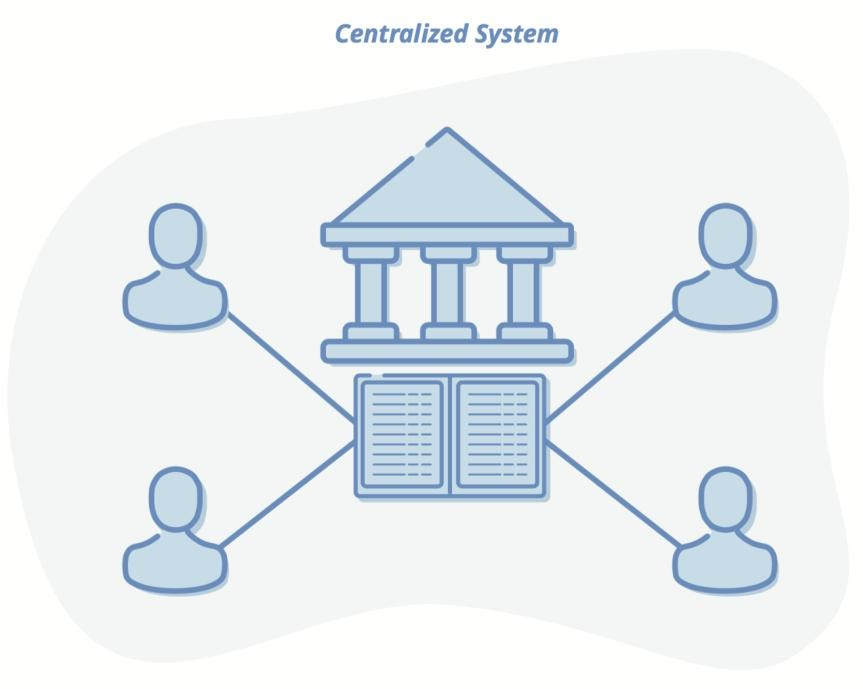
\includegraphics[width=10cm]{imagens/centralizado-capitulo-02.jpg}
  \caption{Sistema centralizado}
\end{figure}


\paragraph{O problema de gasto duplo}
\paragraph{}

O que acontecerá se Ana tentar gastar esses dois dólares novamente? Isso é chamado de problema do gasto duplo. Ela envia a solicitação para o banco, mas o banco diz “Desculpe, vemos que você já gastou R\$2,00 para pagar Bruno, você não tem mais dinheiro para enviar”.

Quando você tem uma autoridade central como um banco, é muito fácil para ele dizer que você está tentando gastar um dinheiro que já gastou. Isso porque eles são os únicos que podem modificar o livro-razão e têm processos internos, incluindo sistemas de backup e auditorias feitas por computadores e seres humanos para se certificar de que está correto e nada foi adulterado.

Chamamos isso de \textit{sistema centralizado} porque possui um único ponto de controle.

\paragraph{Vamos descentralizar o livro razão}
\paragraph{}

O primeiro problema que o Bitcoin visa resolver é a remoção de um intermediário confiável criando um sistema \textit{ponto a ponto}. Vamos imaginar que os bancos desapareceram e precisamos recriar nosso sistema financeiro. Mas desta vez, não vamos ter um ente central. Como podemos manter um livro-razão sem nenhum centralizador?

Se não temos um guardião do livro-razão, precisaremos que o livro-razão pertença ao povo. \textit{Vive la révolution}. É assim que fazemos.

Primeiro, vários de nós nos reunimos e criamos uma \textit{rede}. Isso apenas significa que temos um jeito de conversar uns com os outros. Digamos que trocamos números de telefone ou contas de Snapchat. Quando Ana quiser enviar dinheiro para Bruno, ao invés de ligar para o banco, ela vai no Snapchat de todos os seus amigos e diz a eles: “Estou enviando R\$2,00 para Bruno”. Todos a reconhecem, respondendo "Legal, entendemos!", e escrevem em suas cópias do livro-razão. A imagem agora tem a seguinte aparência:

~

\begin{figure}
  \centering
  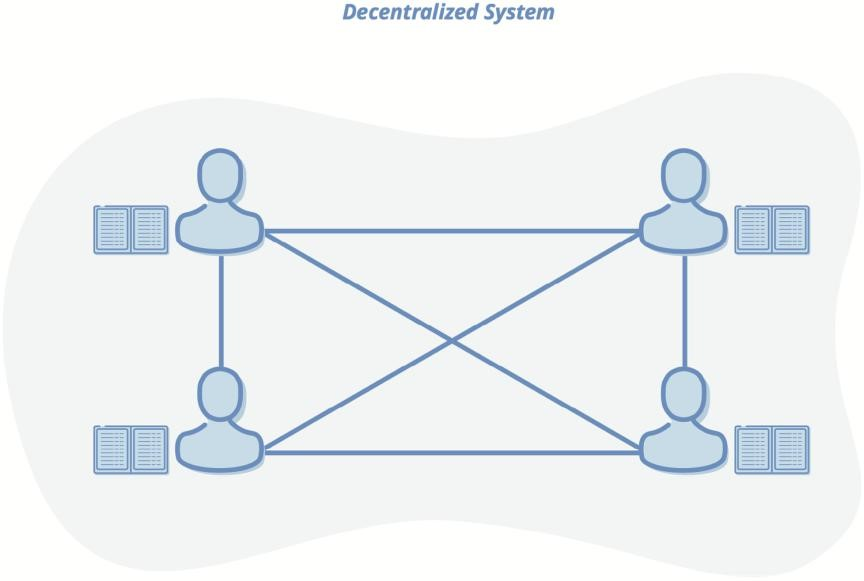
\includegraphics[width=10cm]{imagens/descentralizado-capitulo-02.jpg}
  \caption{Sistema descentralizado}
\end{figure}
\newpage

Portanto, ao invés de um único banco, temos uma cópia do livro-razão nas mãos de todos. Sempre que alguém quer gastar o dinheiro, basta ligar ou fazer um snapchat a todos os seus amigos e informá-los de que isso está acontecendo. Todos registrarão as transações. Como o livro-razão não está mais em apenas um lugar, nós o chamamos de \textit{distribuído} e, como nenhum ente centralizado é responsável, o chamamos de \textit{descentralizado}.

Como isso resolve o problema do gasto duplo? Bem, uma vez que todos possuem uma cópia do livro-razão, se Ana tentar gastar novamente os R\$2,00 que ela já enviou para Bruno, sua transação será rejeitada por todos na rede, já que eles consultariam seus livros-razão e diriam a ela que de acordo com seus registros, ela já gastou o dinheiro.

Agora temos uma rede ponto a ponto para registrar propriedade e transferências de fundos. Este sistema funciona muito bem entre um grupo de amigos que têm motivos sociais para não enganar uns aos outros, mas isso não se aplica quando as redes possuem milhões de pessoas. À medida que mais e mais pessoas começam a usar o sistema, há um incentivo para trapacear para obter dinheiro extra no livro-razão.

Como mantemos todos honestos?